\documentclass[12pt,a4paper]{article}
\usepackage{graphicx}
\usepackage{amsmath}
\usepackage{geometry}
\usepackage{float}
\usepackage{caption} % needed for \captionof
\geometry{margin=1in}

\usepackage{listings}      % Add this to preamble
\usepackage{xcolor}        % Optional, for syntax highlighting

\definecolor{codegray}{rgb}{0.5,0.5,0.5}
\definecolor{codegreen}{rgb}{0,0.6,0}
\definecolor{codepurple}{rgb}{0.58,0,0.82}
\definecolor{backcolour}{rgb}{0.95,0.95,0.95}

\lstdefinestyle{mystyle}{
    backgroundcolor=\color{backcolour},
    commentstyle=\color{codegreen},
    keywordstyle=\color{blue},
    numberstyle=\tiny\color{codegray},
    stringstyle=\color{codepurple},
    basicstyle=\ttfamily\footnotesize,
    breaklines=true,
    breakatwhitespace=true,
    numbers=left,
    numbersep=5pt,
    frame=single,
    tabsize=4
}

\lstset{style=mystyle, language=Matlab}

\title{\textbf{EP3101 Mini Project:} Numerical Simulation of Foucault Pendulum}
\author{Sahil Raj (2301CS41)}
\date{\today}

\begin{document}

\maketitle

\section{Introduction}
This project simulates the motion of a Foucault pendulum numerically using a finite difference
method, accounting for the Coriolis force due to Earth's rotation. The simulation is performed
for a pendulum at different latitudes and earth's angular velocity.

\section{Parameters and Setup}
The parameters used in the simulation are:

\begin{itemize}
    \item Latitude: 25°
    \item Pendulum length ($l$): 1.0 m
    \item Pendulum mass ($m$): 1.0 kg
    \item Gravitational acceleration ($g$): 9.81 m/s\textsuperscript{2}
    \item Time step ($\Delta t$): 0.1 s
    \item Maximum simulation time (T): 3600 s
    \item Earth's angular velocity ($\omega_{0}$): $360/86400$ deg/s
\end{itemize}

\section{Methodology}
The motion of the pendulum is modeled using finite difference approximations. Let $x(t)$ and $y(t)$
be the horizontal displacements of the pendulum. The numerical integration is performed using the
following recurrence relations:

\[
y_i = c_1 y_{i-2} + c_2 y_{i-1} + c_3 x_{i-2} + c_4 x_{i-1}
\]

\[
x_i = c_1 x_{i-2} + c_2 x_{i-1} - c_3 y_{i-2} - c_4 y_{i-1}
\]

where $c_1, c_2, c_3, c_4$ are coefficients depending on the system constants and simulation
parameters.

\section{MATLAB Code}
The following MATLAB code was used to simulate the Foucault pendulum:

\begin{lstlisting}
%% PARAMETERS
LATITUDE = 25;
ANGVAL = 360 / 86400;
G = 9.81;
dt = 0.1;
l = 1.0;
m = 1.0;
T = 3600;

%% CONVERSIONS
lat = deg2rad(LATITUDE);
av = deg2rad(ANGVAL);

%% EFFECTIVE ROTATION COMPONENT
Omeg = av * sin(lat);

%% FINITE DIFFERENCE COEFFICIENTS
phi = (G*dt^2/l - 2);
mu_p = Omeg^2 * dt^2 + 1;
mu_n = Omeg^2 * dt^2 - 1;

c1 = mu_n / mu_p;
c2 = -phi / mu_p;
c3 = 2 * Omeg * dt / mu_p;
c4 = Omeg * dt * phi / mu_p;

%% TIME VECTOR
t = 0:dt:T;
N = length(t);

%% INITIAL CONDITIONS
x = zeros(N, 1);
y = zeros(N, 1);

x(1) = 1.0;
x(2) = 1.0;
y(1) = 0.0;
y(2) = 0.0;

%% NUMERICAL INTEGRATION USING FINITE DIFFERENCE
for i = 3:N
    y(i) = c1 * y(i-2) + c2 * y(i-1) + c3 * x(i-2) + c4 * x(i-1);
    x(i) = c1 * x(i-2) + c2 * x(i-1) - c3 * y(i-2) - c4 * y(i-1);
end

%% PLOT RESULTS
figure;
plot(x, y, 'b', 'LineWidth', 1.5);
grid on;
axis equal;
xlabel('X Displacement (m)');
ylabel('Y Displacement (m)');
title('Foucault Pendulum Trajectory');
\end{lstlisting}


\section{Simulation Results}

\subsection{Case $\omega_1 = \omega_{0}$}
\textbf{NOTE}: Here $\omega_{0}$ is the true angular velocity of earth.
\begin{figure}[H]
    \centering
    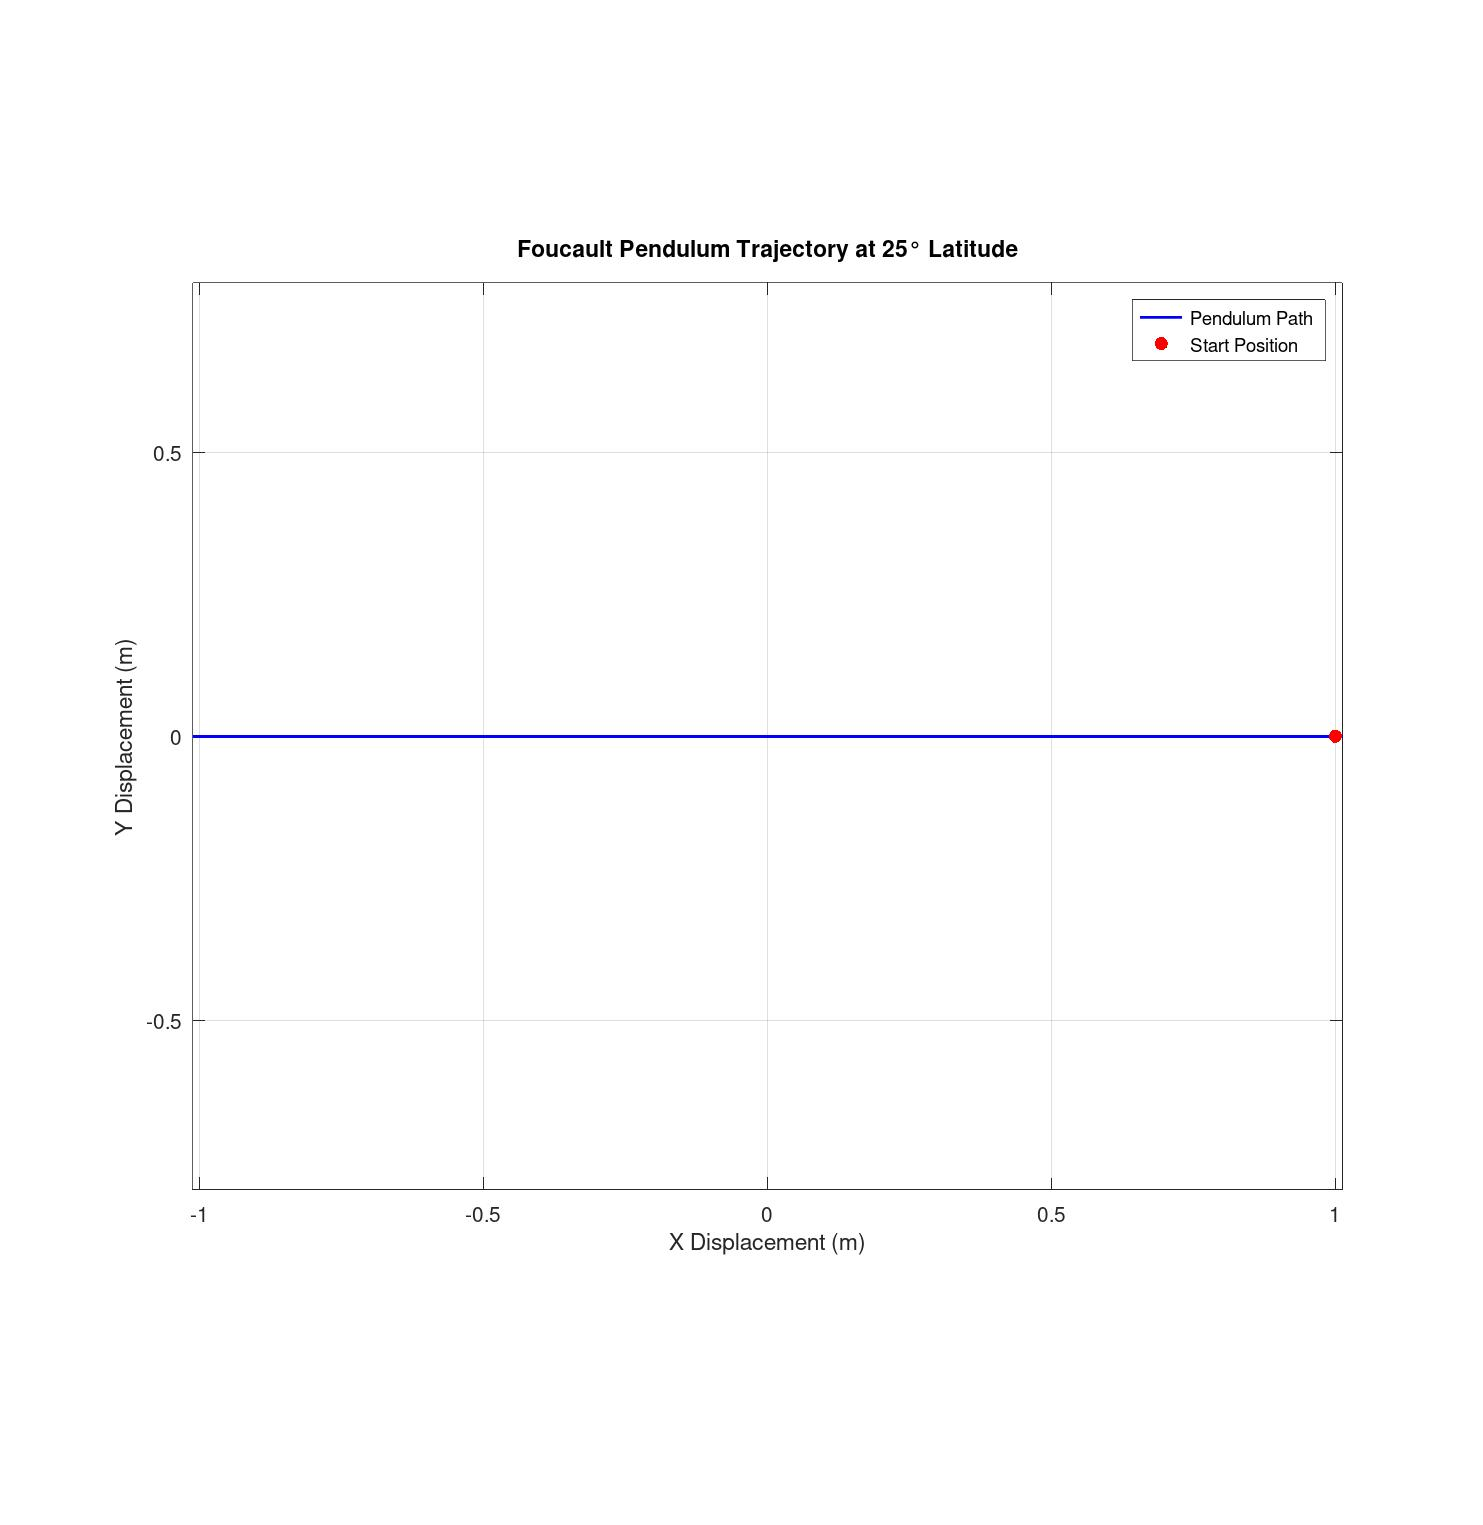
\includegraphics[width=0.32\textwidth]{traj_0.jpg}
    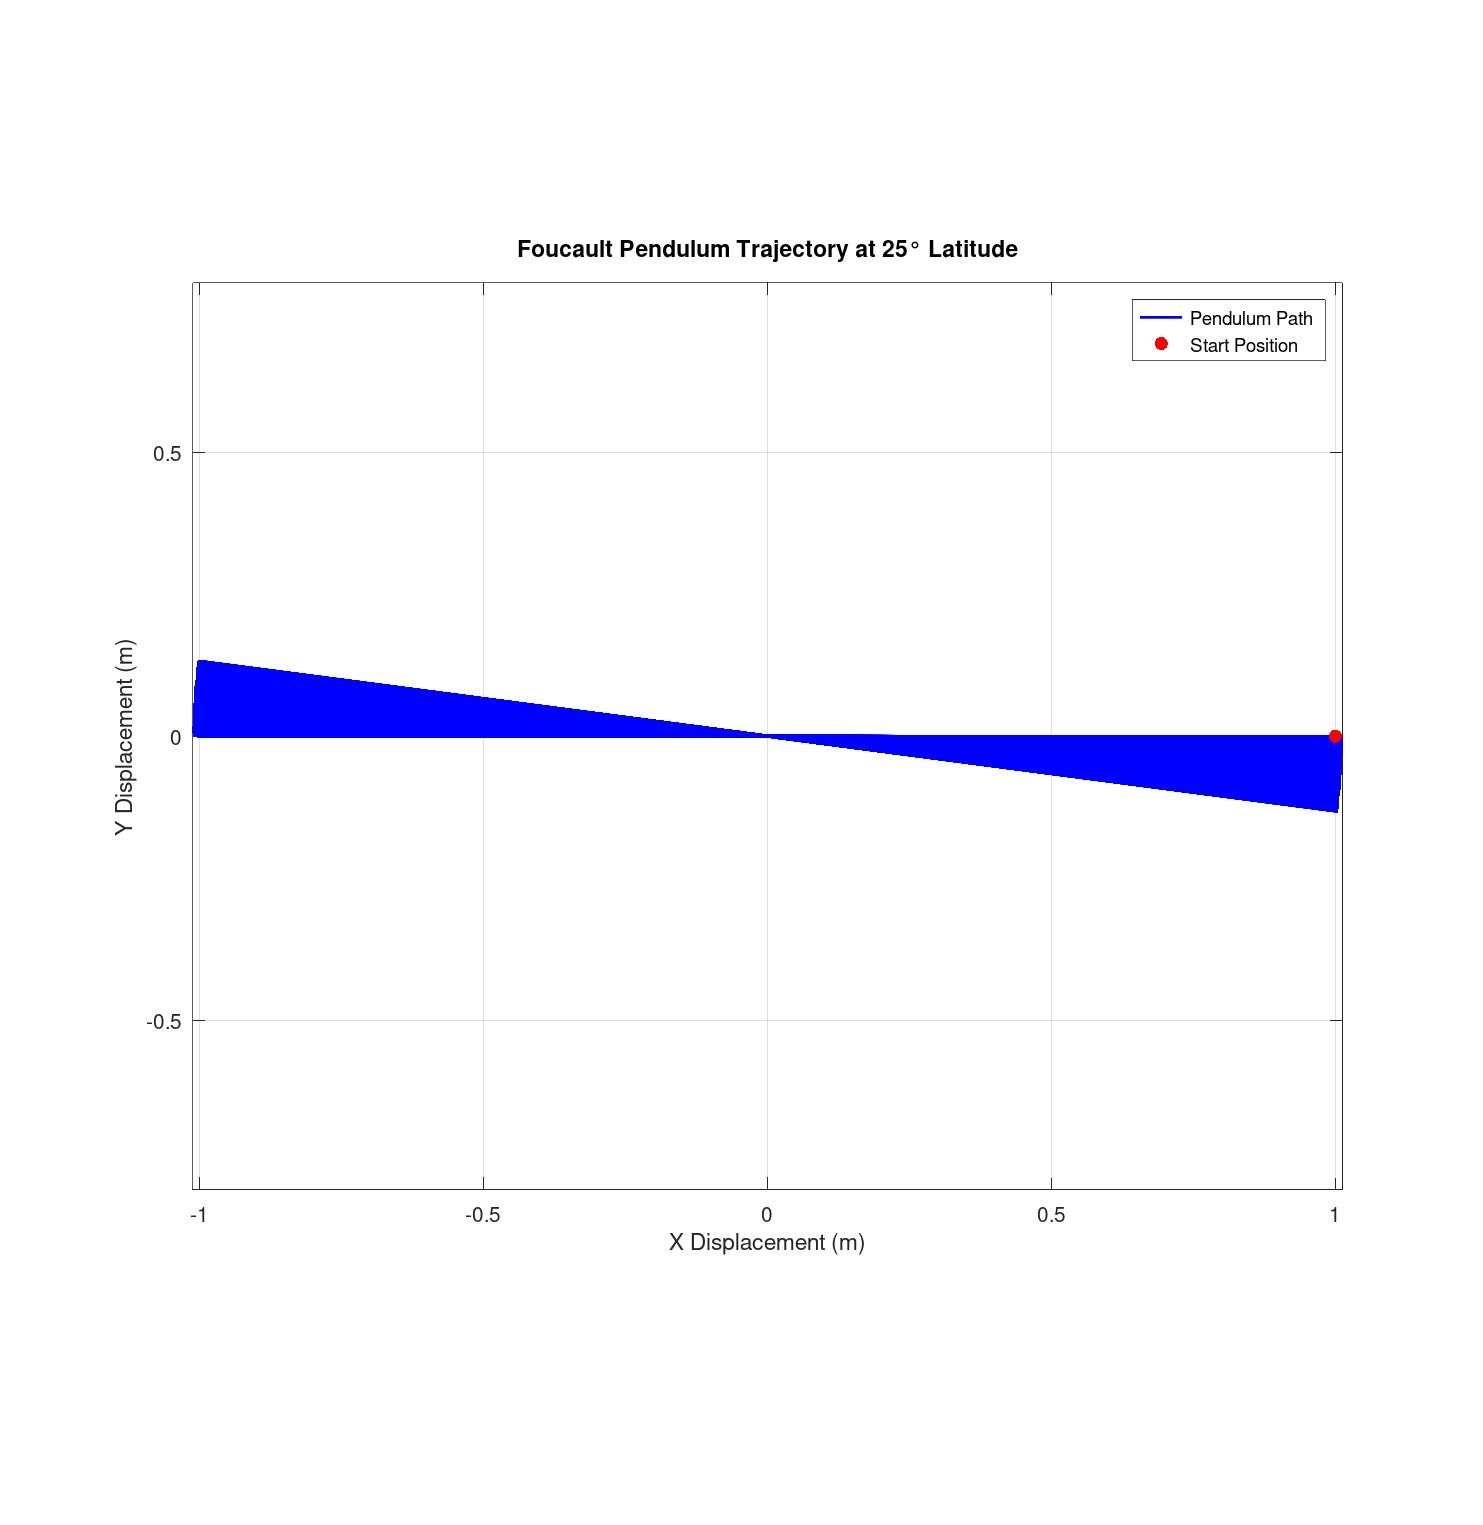
\includegraphics[width=0.32\textwidth]{traj_30.jpg}
    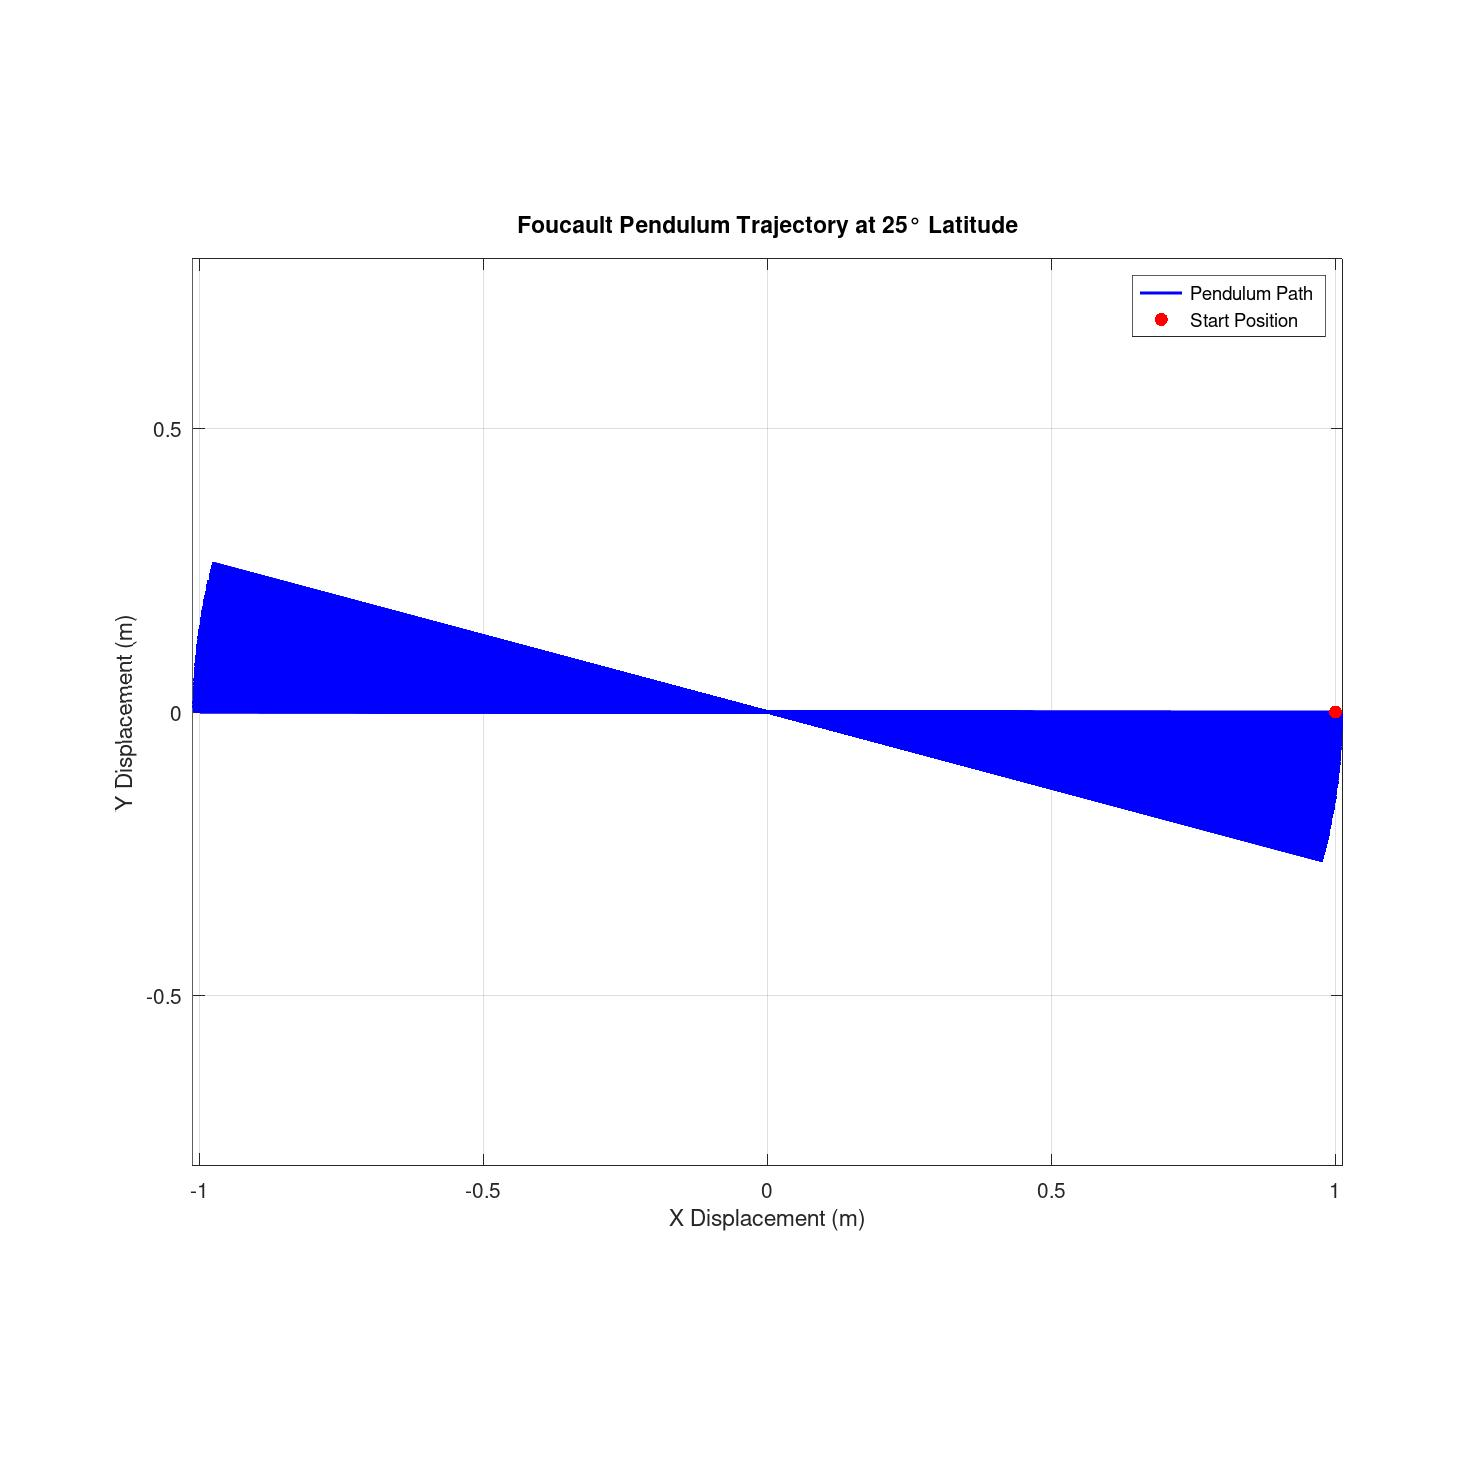
\includegraphics[width=0.32\textwidth]{traj_90.jpg}
    \caption{Pendulum trajectories \textit{(top-view)} for $\omega_1$ with latitudes $\theta = 0^\circ, 30^\circ, 90^\circ$.}
\end{figure}

\subsection{Case $\omega_2 = 10\omega_{0}$}
\begin{figure}[H]
    \centering
    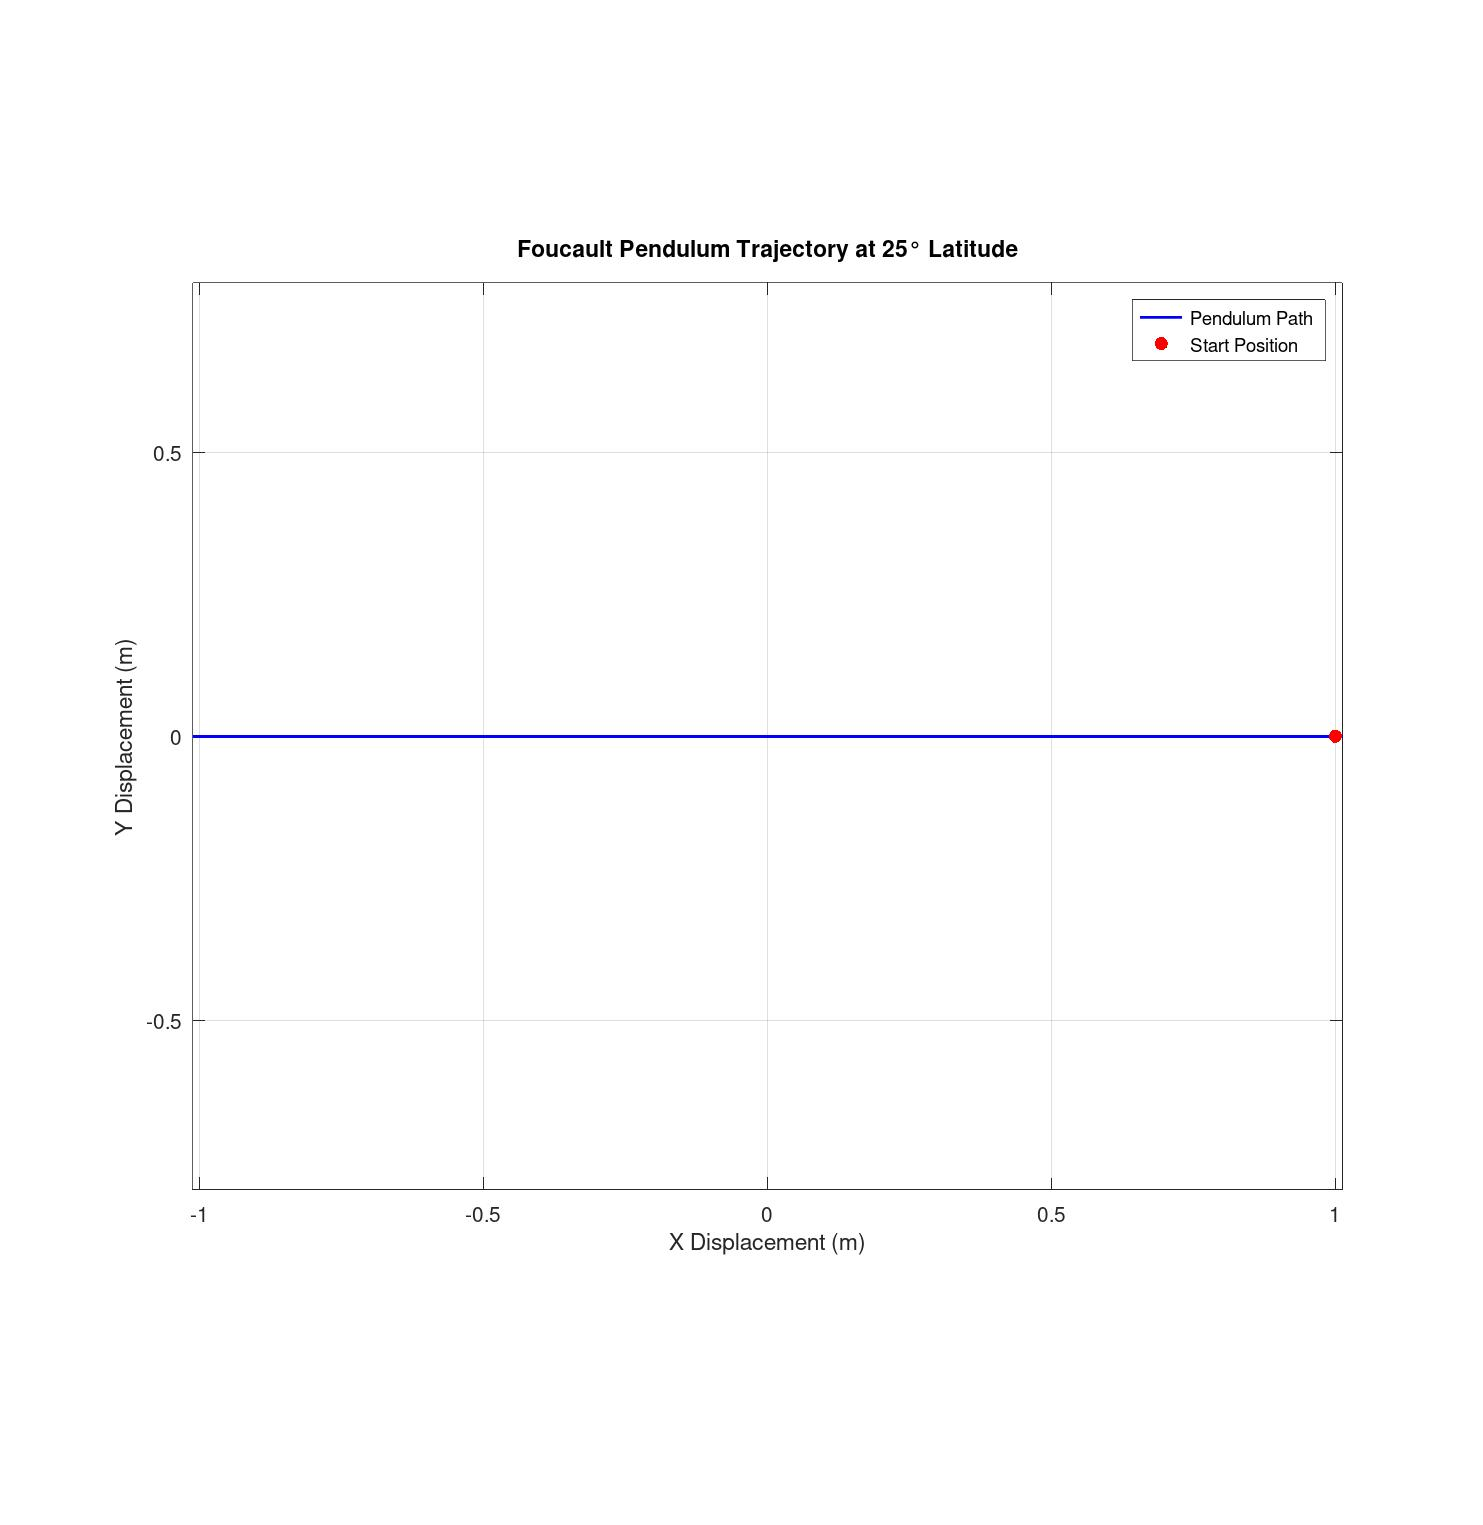
\includegraphics[width=0.32\textwidth]{traj_dec_0.jpg}
    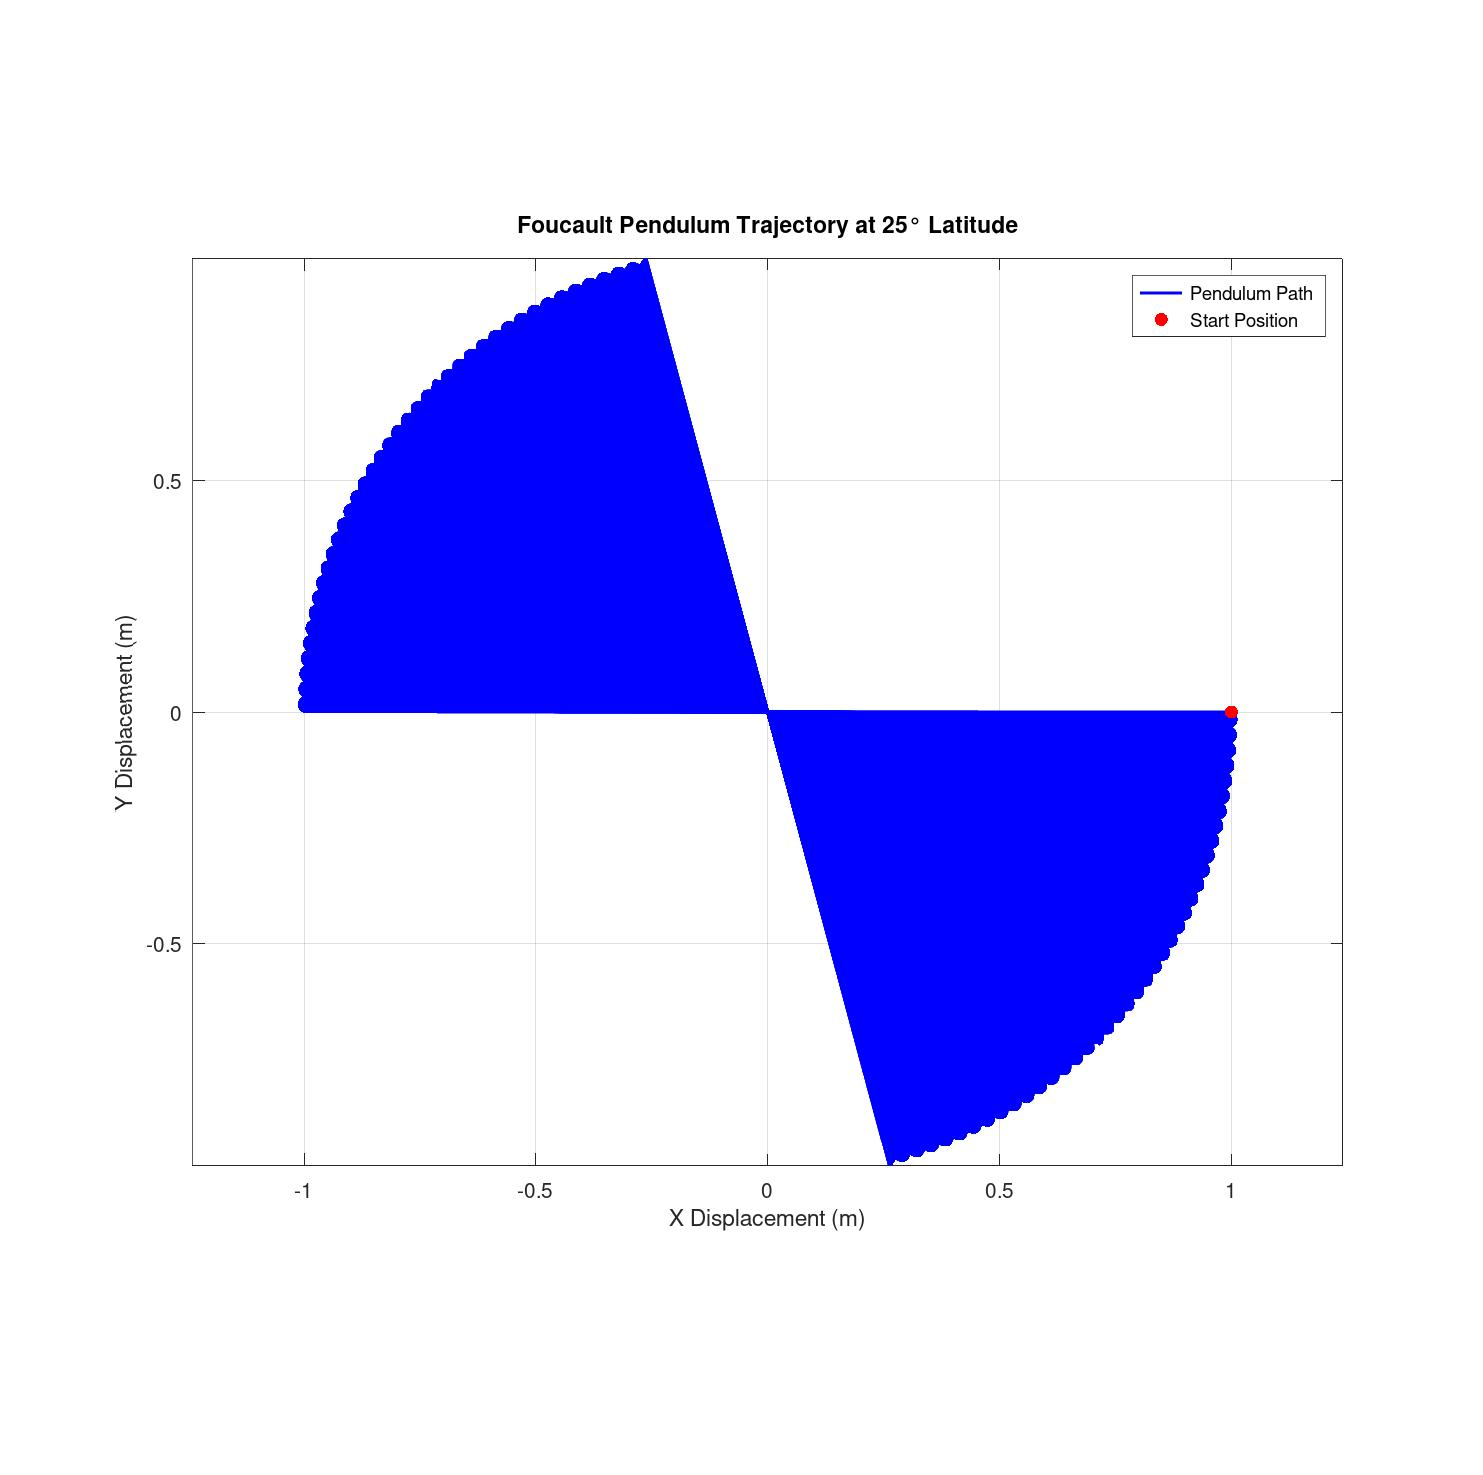
\includegraphics[width=0.32\textwidth]{traj_dec_30.jpg}
    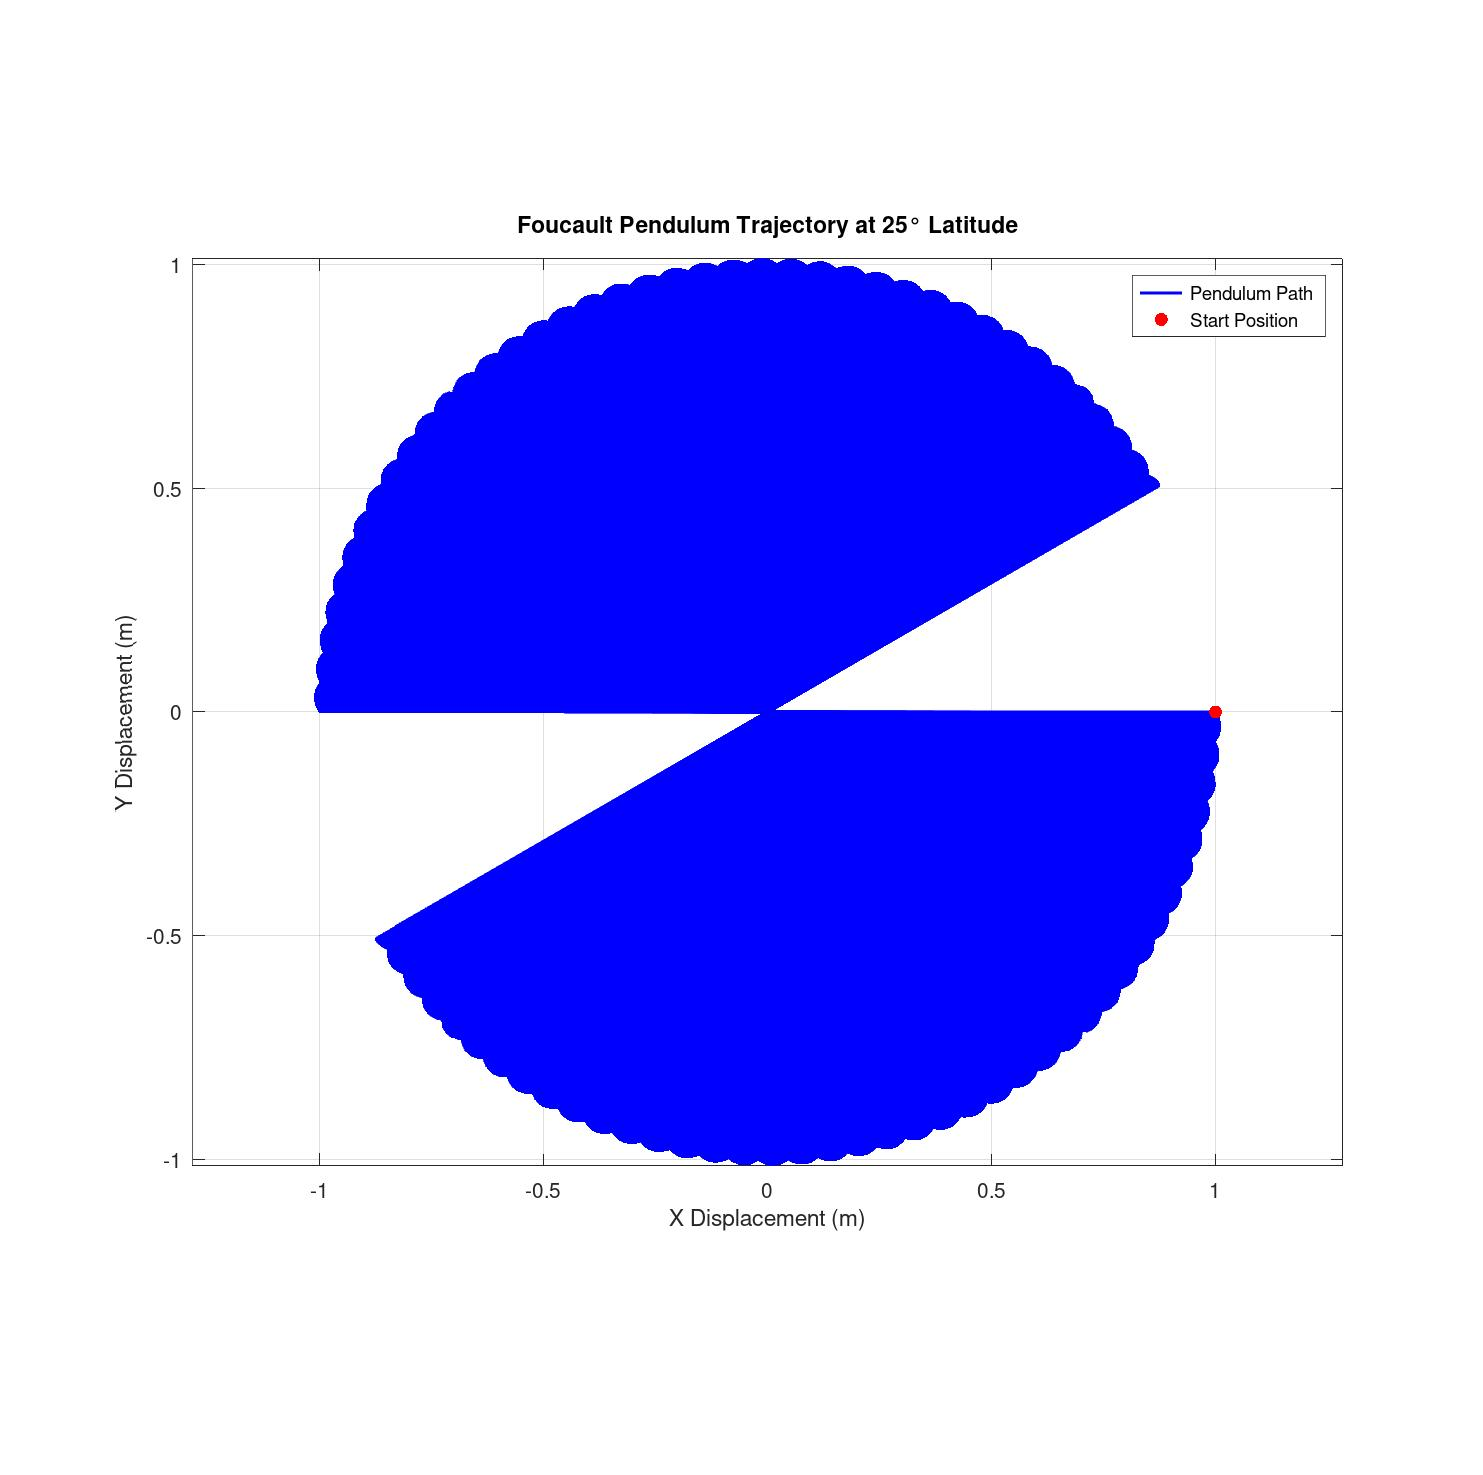
\includegraphics[width=0.32\textwidth]{traj_dec_90.jpg}
    \caption{Pendulum trajectories \textit{(top-view)} for $\omega_2$ with latitudes $\theta = 0^\circ, 30^\circ, 90^\circ$.}
\end{figure}

\section{Calculations}
The numerical calculations for the coefficients are:

\[
\begin{aligned}
\phi &= \frac{G \Delta t^2}{l} - 2 \\
\mu_p &= \Omega^2 \Delta t^2 + 1 \\
\mu_n &= \Omega^2 \Delta t^2 - 1 \\
c_1 &= \frac{\mu_n}{\mu_p}, \quad
c_2 = -\frac{\phi}{\mu_p}, \quad
c_3 = \frac{2 \Omega \Delta t}{\mu_p}, \quad
c_4 = \frac{\Omega \Delta t \phi}{\mu_p}
\end{aligned}
\]

\section{Calculation Steps}

\begin{figure}[H]
    \centering
    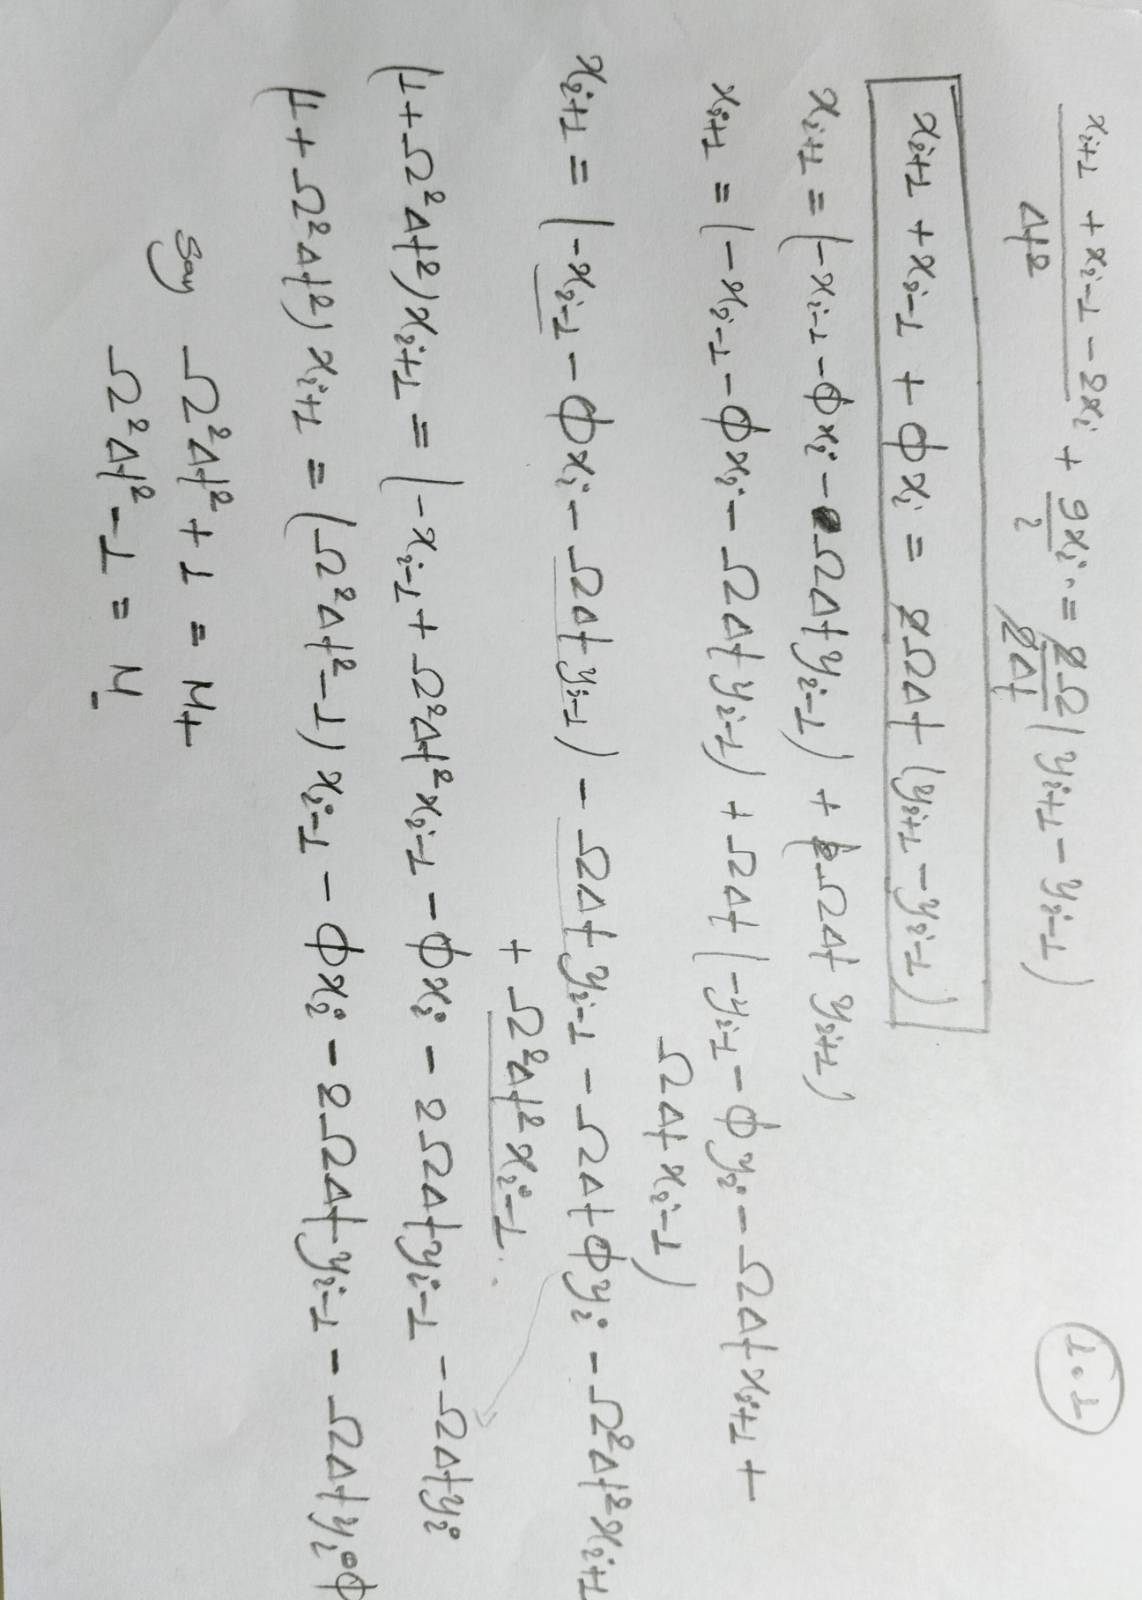
\includegraphics[width=0.7\textwidth,angle=90]{calc1.jpeg}
    \caption{Step 1}
\end{figure}

\begin{figure}[H]
    \centering
    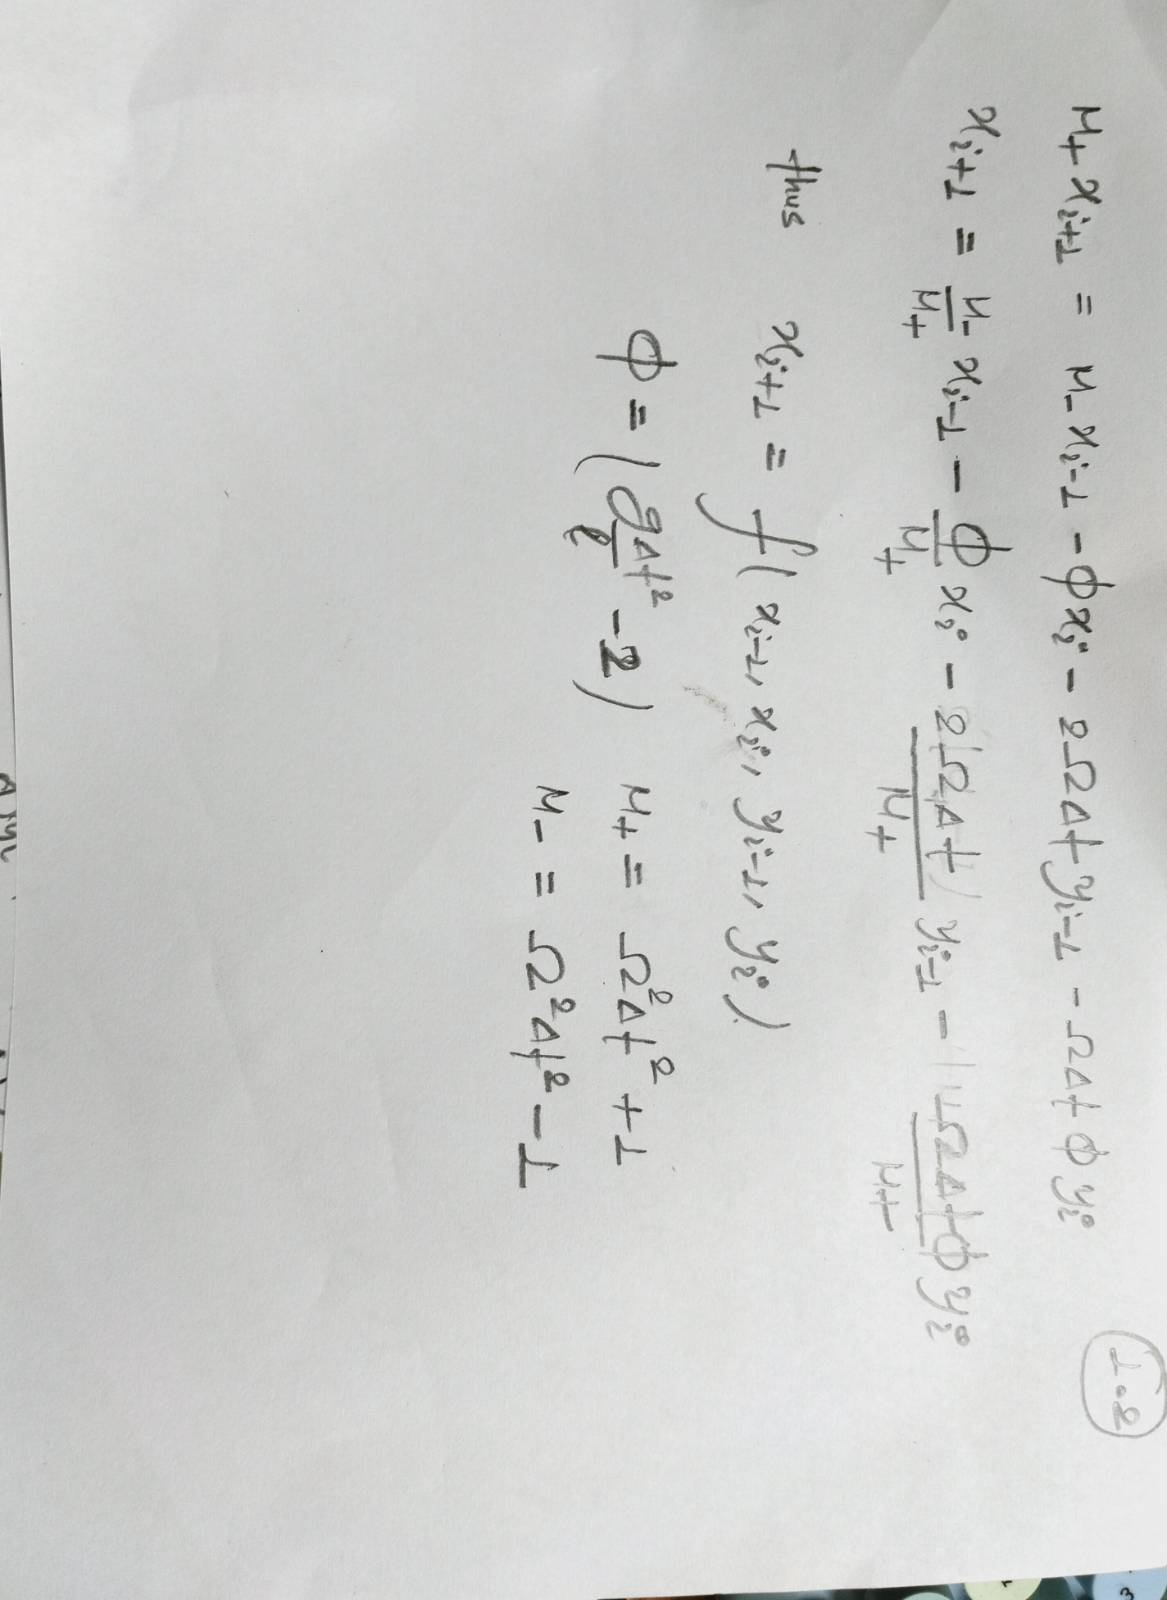
\includegraphics[width=0.7\textwidth,angle=90]{calc2.jpeg}
    \caption{Step 2}
\end{figure}

\begin{figure}[H]
    \centering
    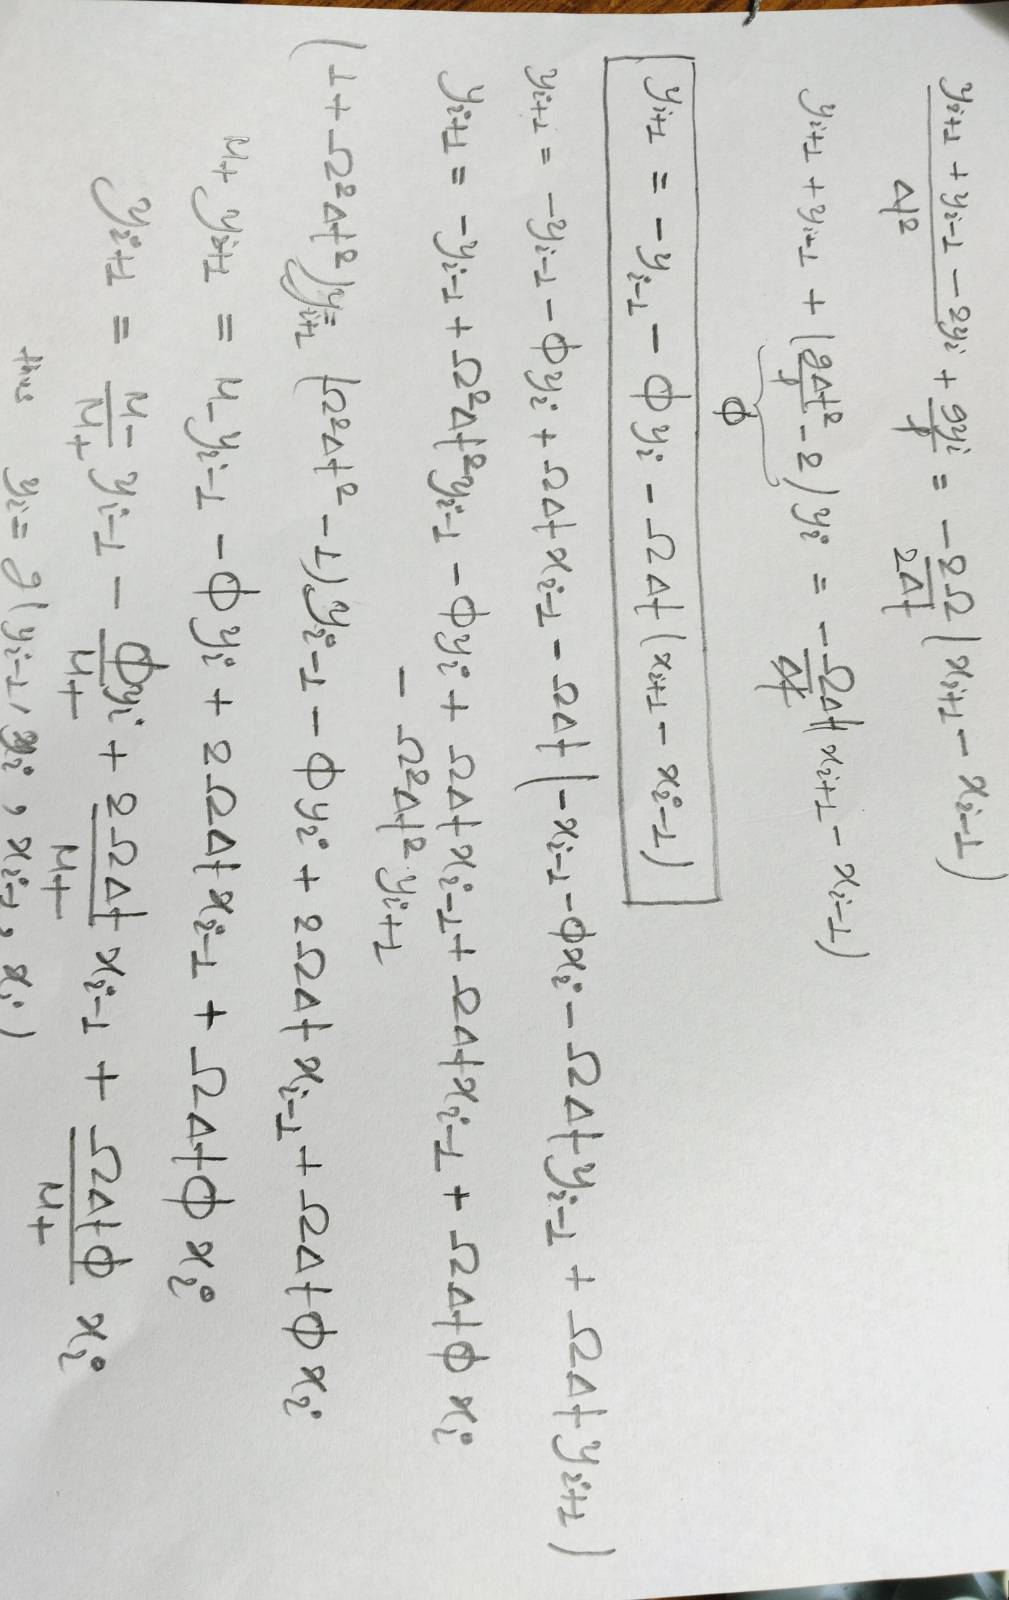
\includegraphics[width=0.7\textwidth,angle=90]{calc3.jpeg}
    \caption{Step 3}
\end{figure}

\begin{figure}[H]
    \centering
    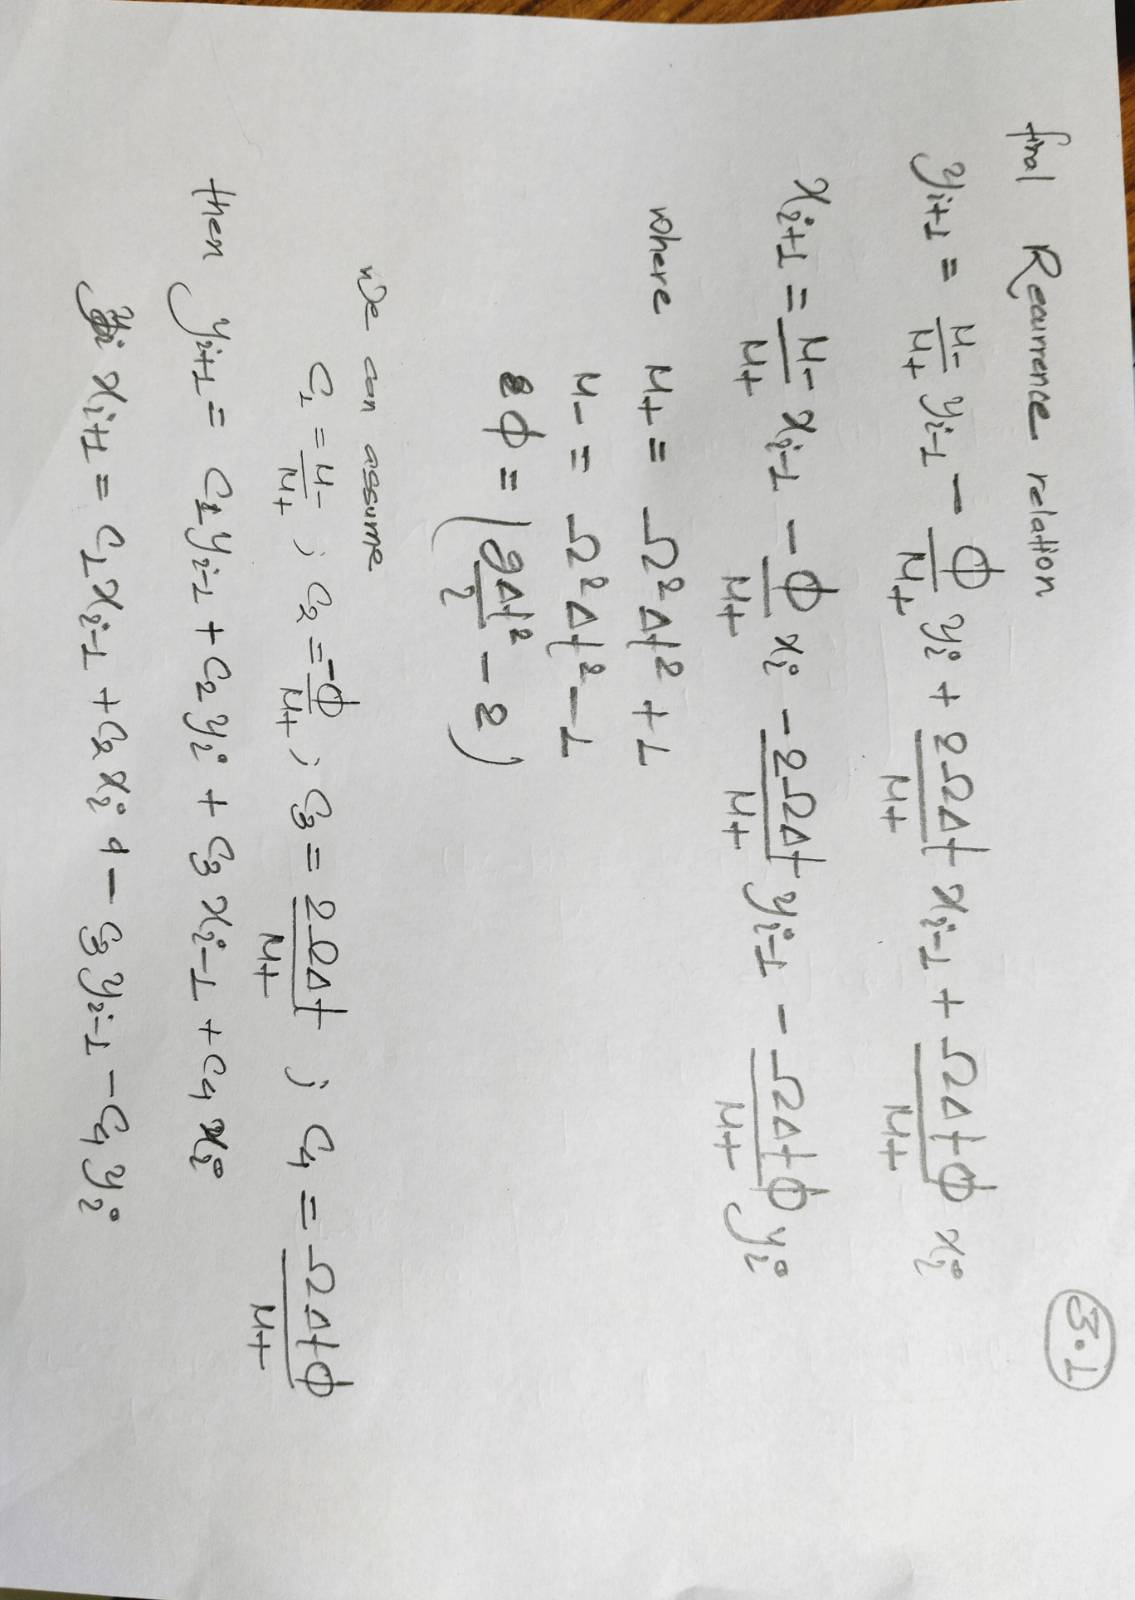
\includegraphics[width=0.7\textwidth,angle=90]{calc4.jpeg}
    \caption{Step 4}
\end{figure}

\begin{figure}[H]
    \centering
    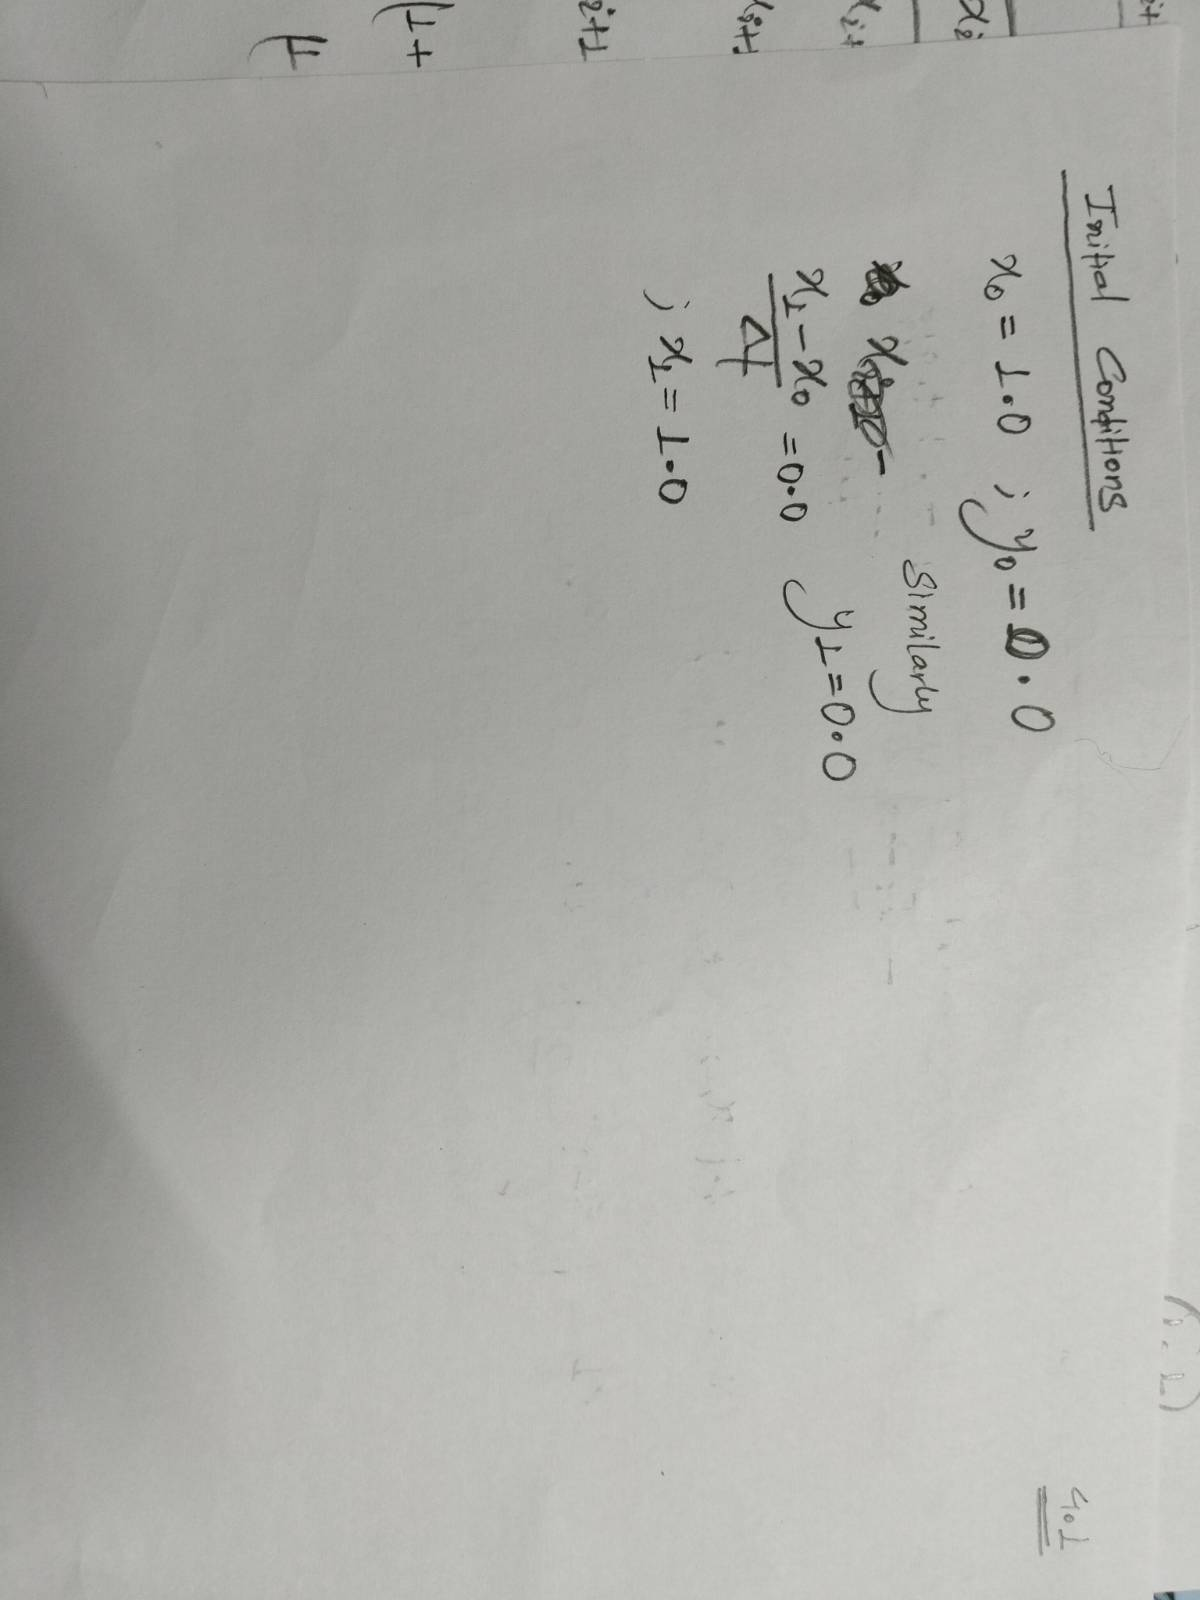
\includegraphics[width=0.7\textwidth,angle=90]{calc5.jpeg}
    \caption{Step 5}
\end{figure}

\section{Conclusion}
The simulation successfully demonstrates the motion of the Foucault pendulum and its precession
due to Earth's rotation. The finite difference method accurately approximates the trajectory. The angle swept
by the pendulum plane increases with latitude angle, and it also increases with increasing $\omega$.
\end{document}
